\documentclass{puzzlehunt}

\usepackage[final]{pdfpages}
\usepackage{amsmath,amssymb}
\usepackage{pgf,tikz}
\usetikzlibrary{arrows}
\usetikzlibrary{lindenmayersystems}
\usetikzlibrary{shapes}


\usepackage{array}

\usepackage{environ}

\usepackage{chessfss}

\usepackage{multicol}
\usepackage{multirow}

\usepackage{wrapfig}
\usepackage{alphalph}
\usepackage{contour}

% \usepackage{pigpen}\renewcommand{\pigpenfont}{} %stopgap for when pigpen fails
\usepackage{pdfpages} % need longer term fix

\usepackage[puttinydots]{braille}



% Contest name macros
\newcommand{\phEventName}{MAA MathFest 2018 - MaPP Challenge DEMO} 
\newcommand{\phEventAbbr}{Challenge18}

\title{\phEventName}
\author{Mathematical Puzzle Programs}
\date{\today}

\parindent=0pt

\newcommand{\mappMobimon}{Mob\'imon}
\newcommand{\mappMobidex}{Mob\'idex}
\newcommand{\mappMobidot}{Mob\`imon}
\newcommand{\mappMobidash}{Mob\^imon}

\newcommand{\blindCrissCrossEntry}[2]{
  \draw[step=1,dotted] #1 grid #2;
  \draw[very thick] #1 rectangle #2
}
\newcommand{\blindCrissCrossPip}[2]{
  \draw[fill=black] (#1.5,#2.5) circle (0.3)
}

\newcommand{\morseDit}{\(\cdot\)}
\newcommand{\morseDah}{\(-\)}


%%%%%%%% \phMarkDraft

\phSetSquareLogo{assets/mapp-square.pdf}
\phSetBannerLogo{assets/mapp-banner.pdf}

\begin{document}

% \frontmatter % roman page numbers

\phTitlePage
% \phTableOfContents

% \mainmatter % arabic page numbers

% FIXME
% \phChapter{Code Sheet}
% %!TEX root =../mapp-challenge-18-game-book.tex
% ^ leave for LaTeXTools build functionality

\begin{center}\small
  \begin{tabular}{c|c|c|c|c}
    Letter &
      Number &
      Morse Code &
      Braille &
      Pig Pen\\\hline
    A &
      1 &
      \morseDit\morseDah &
      \braille{a}&
      {\pigpenfont A}\\
    B &
      2 &
      \morseDah\morseDit\morseDit\morseDit &
      \braille{b}&
      {\pigpenfont B}\\
    C &
      3 &
      \morseDah\morseDit\morseDah\morseDit &
      \braille{c}&
      {\pigpenfont C}\\
    D &
      4 &
      \morseDah\morseDit\morseDit &
      \braille{d}&
      {\pigpenfont D}\\
    E &
      5 &
      \morseDit &
      \braille{e}&
      {\pigpenfont E}\\
    F &
      6 &
      \morseDit\morseDit\morseDah\morseDit &
      \braille{f}&
      {\pigpenfont F}\\
    G &
      7 &
      \morseDah\morseDah\morseDit &
      \braille{g}&
      {\pigpenfont G}\\
    H &
      8 &
      \morseDit\morseDit\morseDit\morseDit &
      \braille{h}&
      {\pigpenfont H}\\
    I &
      9 &
      \morseDit\morseDit &
      \braille{i}&
      {\pigpenfont I}\\
    J &
      10 &
      \morseDit\morseDah\morseDah\morseDah &
      \braille{j}&
      {\pigpenfont J}\\
    K &
      11 &
      \morseDah\morseDit\morseDah &
      \braille{k}&
      {\pigpenfont K}\\
    L &
      12 &
      \morseDit\morseDah\morseDit\morseDit &
      \braille{l}&
      {\pigpenfont L}\\
    M &
      13 &
      \morseDah\morseDah &
      \braille{m}&
      {\pigpenfont M}\\
    N &
      14 &
      \morseDah\morseDit &
      \braille{n}&
      {\pigpenfont N}\\
    O &
      15 &
      \morseDah\morseDah\morseDah &
      \braille{o}&
      {\pigpenfont O}\\
    P &
      16 &
      \morseDit\morseDah\morseDah\morseDit &
      \braille{p}&
      {\pigpenfont P}\\
    Q &
      17 &
      \morseDah\morseDah\morseDit\morseDah &
      \braille{q}&
      {\pigpenfont Q}\\
    R &
      18 &
      \morseDit\morseDah\morseDit &
      \braille{r}&
      {\pigpenfont R}\\
    S &
      19 &
      \morseDit\morseDit\morseDit &
      \braille{s}&
      {\pigpenfont S}\\
    T &
      20 &
      \morseDah &
      \braille{t}&
      {\pigpenfont T}\\
    U &
      21 &
      \morseDit\morseDit\morseDah &
      \braille{u}&
      {\pigpenfont U}\\
    V &
      22 &
      \morseDit\morseDit\morseDit\morseDah &
      \braille{v}&
      {\pigpenfont V}\\
    W &
      23 &
      \morseDit\morseDah\morseDah &
      \braille{w}&
      {\pigpenfont W}\\
    X &
      24 &
      \morseDah\morseDit\morseDit\morseDah &
      \braille{x}&
      {\pigpenfont X}\\
    Y &
      25 &
      \morseDah\morseDit\morseDah\morseDah &
      \braille{y}&
      {\pigpenfont Y}\\
    Z &
      26 &
      \morseDah\morseDah\morseDit\morseDit &
      \braille{z}&
      {\pigpenfont Z}\\
  \end{tabular}
\end{center}

\normalsize

%%% Local Variables:
%%% mode: latex
%%% TeX-master: "../mapp-hsc17-game-book"
%%% End:


\phPart{Player Handout}

\phChapter{About \& How to Play}

\phSection{About MaPP}

Thanks so much for your interest in
\textbf{Mathematical Puzzle Programs}! Rather than
just tell you what we're about, we thought you'd like to
experience the fun mathematical problem-solving for yourself.

The demo you'll experience in this workshop is a shortened
version of our MaPP Challenge puzzlehunt for 7th-12th
grade students, including puzzles that expose these students
to concepts based on knot theory, combinatorics, and
axiomatic systems. After trying it for yourself, we hope
you'll be interested in partnering with us to bring this
fun mathematical experience to your own community.
If so, be sure to chat with one of the MaPP directors
before you go
or email us at \texttt{info@mappmath.org}! 

\phSection{Teams}

We will organize participants into teams of roughly
2-4 players each. You will complete a walk-around
opening puzzle, followed by four puzzles designed
to be completed together at a table.

The actual game is designed to support
teams of 4-8 students each. Students are usually
provided a classroom where they can openly collaborate
with each other.

\phSection{ClueKeeper app}

We use the ClueKeeper app make playing (and running!)
our mathematical puzzlehunts a breeze.
None of the puzzles printed in this packet can be
solved alone, but as players progress through the game,
the ClueKeeper app delivers information required
to reveal their hidden meanings.

One member of your team should do the following:

\begin{itemize}
\item Download the app on your iOS or Android device
  at \phUrl{http://cluekeeper.com}. 
\item Open the app, connect it with a Google account
  (or play as a guest), tap ``Enter Hunt Code'', and enter
  a six-character code provided by a MaPP director.
\item Optionally, other members of the team can also install the
app and connect it with a Google account. The user who
entered the Hunt Code into their app can add these additional
teammates using the menu in the corner of the app.
\end{itemize}


When your team is ready, use the code \textbf{DEMO}
  to start the game!

\includepdf{overview/code-sheet.pdf}

%!TEX root =../mapp-challenge-18-game-book.tex
% ^ leave for LaTeXTools build functionality

\phChapterWorksheet{Gotta Solve 'Em All!}{Teaser Puzzle}

In \phEventName{}, your team will travel to the world of
\textbf{\mappMobimon{}}, where trainers befriend monsters and battle them
against their opponents!
(Now where have I heard that idea before?...) Of course, you'll probably
find yourself encountering a wild \textbf{puzzle} or two, so let's see how
you deal with this conundrum...

In a previous \mappMobimon{} tournament, six trainers competed and were
ranked 1st through 6th: Ash, Brock, Cynthia, Drayden, Erika, and Flannery.
You have been told the following facts about these results:

\begin{multicols}{3}\footnotesize
  \begin{center}
    \includegraphics[width=1.2in]{assets/unknot1.pdf}

    Ash and Flannery did not place 6th.


    \includegraphics[width=1.2in]{assets/knot1.pdf}

    Neither Brock nor Drayden placed 4th.


    \includegraphics[width=1.2in]{assets/unknot2.pdf}

    Erika placed exactly one rank higher than Ash.


    \includegraphics[width=1.2in]{assets/knot2.pdf}

    Drayden placed in the top three.


    \includegraphics[width=1.2in]{assets/knot3.pdf}

    Brock placed lower than Flannery.


    \includegraphics[width=1.2in]{assets/unknot3.pdf}

    Either Cynthia or Drayden placed 3rd.
  \end{center}
\end{multicols}

Unfortunately, there's no way all of those claims are \textbf{truthful}.
By inspecting the \textbf{Trainer Badge} above each statement, you can uncover
the \textbf{lies} by deciding if the cord depicted in its design would
\textbf{tighten into a knot} if pulled taut. By blacking out the incorrect
results below, you'll reveal the answer to this riddle: \textit{what is a
mathematician's favorite kind of knot?}

\begin{center}\footnotesize
\begin{tikzpicture}[x=0.2in,y=0.2in]
  \draw[thick] (0,0) rectangle (6,6);
  \draw[step=1] (0,0) grid (6,6);
  \node[anchor=south] at (0.5,6) {\rotatebox{90}{Ash}};
  \node[anchor=south] at (1.5,6) {\rotatebox{90}{Brock}};
  \node[anchor=south] at (2.5,6) {\rotatebox{90}{Cynthia}};
  \node[anchor=south] at (3.5,6) {\rotatebox{90}{Drayden}};
  \node[anchor=south] at (4.5,6) {\rotatebox{90}{Erika}};
  \node[anchor=south] at (5.5,6) {\rotatebox{90}{Flannery}};
  \node[anchor=east] at (0,5.5) {1st};
  \node[anchor=east] at (0,4.5) {2nd};
  \node[anchor=east] at (0,3.5) {3rd};
  \node[anchor=east] at (0,2.5) {4th};
  \node[anchor=east] at (0,1.5) {5th};
  \node[anchor=east] at (0,0.5) {6th};
  \foreach \letters [count=\i] in {
    {O,Y,G,U,S,J},
    {Q,C,M,V,A,X},
    {F,P,U,N,I,E},
    {L,A,S,I,D,T},
    {K,N,B,Z,T,R},
    {H,R,W,E,L,M},
  } {
    \foreach \letter [count=\j] in \letters {
      \node at ($(\j.5,-\i.5)+(-1,7)$) {\letter};
    }
  }
\end{tikzpicture}
\end{center}


\phWorksheet{Teaser Puzzle Solution}

The following cords wouldn't tighten into a knot, so their clues are
\textbf{true}.

\begin{multicols}{3}\footnotesize
  \begin{center}
    \includegraphics[width=1.2in]{assets/unknot1.pdf}

    Ash and Flannery did not place 6th.


    \includegraphics[width=1.2in]{assets/unknot2.pdf}

    Erika placed exactly one rank higher than Ash.


    \includegraphics[width=1.2in]{assets/unknot3.pdf}

    Either Cynthia or Drayden placed 3rd.
  \end{center}
\end{multicols}

The following cords would tighten into a knot, so their clues are
\textbf{false}.

\begin{multicols}{3}\footnotesize
  \begin{center}
    \includegraphics[width=1.2in]{assets/knot1.pdf}

    \textit{Neither Brock nor Drayden placed 4th.}
    Corrected: Either Brock or Drayden placed 4th.


    \includegraphics[width=1.2in]{assets/knot2.pdf}

    \textit{Drayden placed in the top three.}
    Corrected: Drayden placed in the bottom three.


    \includegraphics[width=1.2in]{assets/knot3.pdf}

    \textit{Brock placed lower than Flannery.}
    Corrected: Brock placed higher than Flannery.
  \end{center}
\end{multicols}

Logically, this results in the following grid.

\begin{center}\footnotesize
\begin{tikzpicture}[x=0.2in,y=0.2in]
  \draw[thick,fill=black!80] (0,0) rectangle (6,6);
  \draw[step=1] (0,0) grid (6,6);
  \node[anchor=south] at (0.5,6) {\rotatebox{90}{Ash}};
  \node[anchor=south] at (1.5,6) {\rotatebox{90}{Brock}};
  \node[anchor=south] at (2.5,6) {\rotatebox{90}{Cynthia}};
  \node[anchor=south] at (3.5,6) {\rotatebox{90}{Drayden}};
  \node[anchor=south] at (4.5,6) {\rotatebox{90}{Erika}};
  \node[anchor=south] at (5.5,6) {\rotatebox{90}{Flannery}};
  \node[anchor=east] at (0,5.5) {1st};
  \node[anchor=east] at (0,4.5) {2nd};
  \node[anchor=east] at (0,3.5) {3rd};
  \node[anchor=east] at (0,2.5) {4th};
  \node[anchor=east] at (0,1.5) {5th};
  \node[anchor=east] at (0,0.5) {6th};
  \foreach \letters [count=\i] in {
    {O,Y,G,U,S,J},
    {Q,C,M,V,A,X},
    {F,P,U,N,I,E},
    {L,A,S,I,D,T},
    {K,N,B,Z,T,R},
    {H,R,W,E,L,M},
  } {
    \foreach \letter [count=\j] in \letters {
      \node at ($(\j.5,-\i.5)+(-1,7)$) {\letter};
    }
  }
  \node[circle,inner sep=2pt,draw,fill=white] at (4.5,5.5) {S};
  \node[circle,inner sep=2pt,draw,fill=white] at (0.5,4.5) {Q};
  \node[circle,inner sep=2pt,draw,fill=white] at (2.5,3.5) {U};
  \node[circle,inner sep=2pt,draw,fill=white] at (1.5,2.5) {A};
  \node[circle,inner sep=2pt,draw,fill=white] at (5.5,1.5) {R};
  \node[circle,inner sep=2pt,draw,fill=white] at (3.5,0.5) {E};
\end{tikzpicture}
\end{center}

A mathematican's favorite knot is a \texttt{SQUARE} knot! Oh... you say
you've heard that one before? Well, our \textbf{puzzles} are better than our \textbf{jokes} at the \textbf{MaPP Challenge}, so we hope to see you there!


% Include below for aucTeX integration
%%% Local Variables:
%%% mode: latex
%%% TeX-master: "../mapp-challenge-18-game-book"
%%% End:


% %main puzzles
%!TEX root =../mapp-challenge-18-game-book.tex
% ^ leave for LaTeXTools build functionality

\phChapterWorksheet{When Push Comes to Shove}{Main Puzzle 2}

\newcommand{\mappBoxRow}[2]{
  \fill[color=lightgray] #1 rectangle #2;
  \draw[step=1]          #1 grid #2;
}

% http://oeis.org/A000041 number of partitions
% http://oeis.org/A000009 number of odd/distinct partitions

While training your \mappMobimon{} on Road \(\sqrt{9^2+12^2}\), you are
approached
by \textbf{Dockworker Dave}, who challenges you to a \mappMobimon{} battle!
Of course you accept... turning him down would be \textbf{rude},
don't you think?

It's a close match, but you win! As Dave gives you your victory money, he
tells you about a group of \textbf{Tattarat} \mappMobimon{} that infest the
warehouse he works in. These obnoxious critters like to
\textbf{rearrange the boxes} in his warehouse, so Dave cuts you a deal.
He'll let you catch a Tattarat for your team, but only if you help
him reorganize his boxes.

The boxes in the warehouse must be \textbf{stacked} so that
each row of boxes is always pressed up against the \textbf{left wall} of the
warehouse, and each row of boxes must have the \textbf{same or less boxes} than
every lower row.

Other than that, it's up to you. For example, there are \textbf{seven}
different ways to stack \textbf{five} boxes.

\begin{center}
  \begin{tikzpicture}[x=0.15in,y=0.15in]
    \mappBoxRow{(0,0)}{(5,1)}

    \draw[thick] (0,0) -- (0, 5);
    \draw[thick] (0,0) -- (5, 0);
  \end{tikzpicture}
  \begin{tikzpicture}[x=0.15in,y=0.15in]
    \mappBoxRow{(0,0)}{(4,1)}
    \mappBoxRow{(0,1)}{(1,2)}

    \draw[thick] (0,0) -- (0, 5);
    \draw[thick] (0,0) -- (5, 0);
  \end{tikzpicture}
  \begin{tikzpicture}[x=0.15in,y=0.15in]
    \mappBoxRow{(0,0)}{(3,1)}
    \mappBoxRow{(0,1)}{(2,2)}

    \draw[thick] (0,0) -- (0, 5);
    \draw[thick] (0,0) -- (5, 0);
  \end{tikzpicture}
  \begin{tikzpicture}[x=0.15in,y=0.15in]
    \mappBoxRow{(0,0)}{(3,1)}
    \mappBoxRow{(0,1)}{(1,2)}
    \mappBoxRow{(0,2)}{(1,3)}

    \draw[thick] (0,0) -- (0, 5);
    \draw[thick] (0,0) -- (5, 0);
  \end{tikzpicture}
  \begin{tikzpicture}[x=0.15in,y=0.15in]
    \mappBoxRow{(0,0)}{(2,1)}
    \mappBoxRow{(0,1)}{(2,2)}
    \mappBoxRow{(0,2)}{(1,3)}

    \draw[thick] (0,0) -- (0, 5);
    \draw[thick] (0,0) -- (5, 0);
  \end{tikzpicture}
  \begin{tikzpicture}[x=0.15in,y=0.15in]
    \mappBoxRow{(0,0)}{(2,1)}
    \mappBoxRow{(0,1)}{(1,2)}
    \mappBoxRow{(0,2)}{(1,3)}
    \mappBoxRow{(0,3)}{(1,4)}

    \draw[thick] (0,0) -- (0, 5);
    \draw[thick] (0,0) -- (5, 0);
  \end{tikzpicture}
  \begin{tikzpicture}[x=0.15in,y=0.15in]
    \mappBoxRow{(0,0)}{(1,1)}
    \mappBoxRow{(0,1)}{(1,2)}
    \mappBoxRow{(0,2)}{(1,3)}
    \mappBoxRow{(0,3)}{(1,4)}
    \mappBoxRow{(0,4)}{(1,5)}

    \draw[thick] (0,0) -- (0, 5);
    \draw[thick] (0,0) -- (5, 0);
  \end{tikzpicture}
\end{center}

The dockworker notices your good work.
``Hey, didya say you were aiming to become one of them \mappMobimon{}
Champions? Maybe you're smart enough to solve this \textbf{puzzle} for me
then.'' It seems that if you can count the following different combinations
of stacked boxes, you'll be able to reveal a \textbf{hidden message} by
converting the numbers to appropriate letters (A=1, B=2, and so on).

\begin{multicols}{2}
  \begin{itemize}
    \item %M=13
      The number of ways you can stack either \(2\) or \(6\) boxes.
    \item %O=15
      The number of ways you can stack \(12\) boxes, if every row must
      contain an odd number.
    \item %U=21
      The number of ways you can stack \(8\) boxes, if every row must contain
      less than eight.
    \item %S=19
      The number of ways you can stack up to \(5\) boxes. (An empty room
      counts as one way...)
    \item %E=5
      The number of ways you can stack \(4\) boxes.
  \end{itemize}
\columnbreak
  \begin{itemize}
    \item %T=20
      The number of ways you can stack \(8\) boxes, if every row must contain
      less than seven.
    \item %R=18
      The number of ways you can stack \(13\) boxes, if every row must have
      less boxes than the row below it.
    \item %A=1
      The number of ways you can stack \(42\) boxes, if you can only use one
      row.
    \item %P=16
      The number of ways you can stack \(1\) or \(12\) boxes, if every row must
      have a unique number of boxes.
  \end{itemize}
\end{multicols}


%%SOLUTION%%%
% MOUSETRAP %
%%%%%%%%%%%%%


% Old unused text:

% For example, this configuration looks solid.
% \begin{center}
%   \begin{tikzpicture}
%     \fill[color=lightgray] (0,0) rectangle (4,1);
%     \draw             (0,0) grid (4,1);
%     \fill[color=lightgray] (0,1) rectangle (3,2);
%     \draw             (0,1) grid (3,2);
%     \fill[color=lightgray] (0,2) rectangle (1,3);
%     \draw             (0,2) grid (1,3);
%
%     \draw[thick] (0,0) -- (0, 4);
%     \draw[thick] (0,0) -- (5, 0);
%   \end{tikzpicture}
% \end{center}
%
% But this one isn't so great.
% Not only are the boxes not all pushed to the left, but how are some of them
% floating in the air like that anyway? That's just not right.
%
% \begin{center}
%   \begin{tikzpicture}
%     \fill[color=lightgray] (0,0) rectangle (2,1);
%     \draw             (0,0) grid (2,1);
%     \fill[color=lightgray] (1,1) rectangle (4,2);
%     \draw             (1,1) grid (4,2);
%     \fill[color=lightgray] (2,2) rectangle (3,3);
%     \draw             (2,2) grid (3,3);
%
%     \draw[thick] (0,0) -- (0,4);
%     \draw[thick] (0,0) -- (5,0);
%   \end{tikzpicture}
% \end{center}
%




%%% Local Variables:
%%% mode: latex
%%% TeX-master: "../mapp-challenge-18-game-book"
%%% End:

%!TEX root =../mapp-challenge-18-game-book.tex
% ^ leave for LaTeXTools build functionality

\phChapterWorksheet{The Nickname Rater}{Popular Nicknames}
% https://en.wikipedia.org/wiki/MU_puzzle

\begin{center}
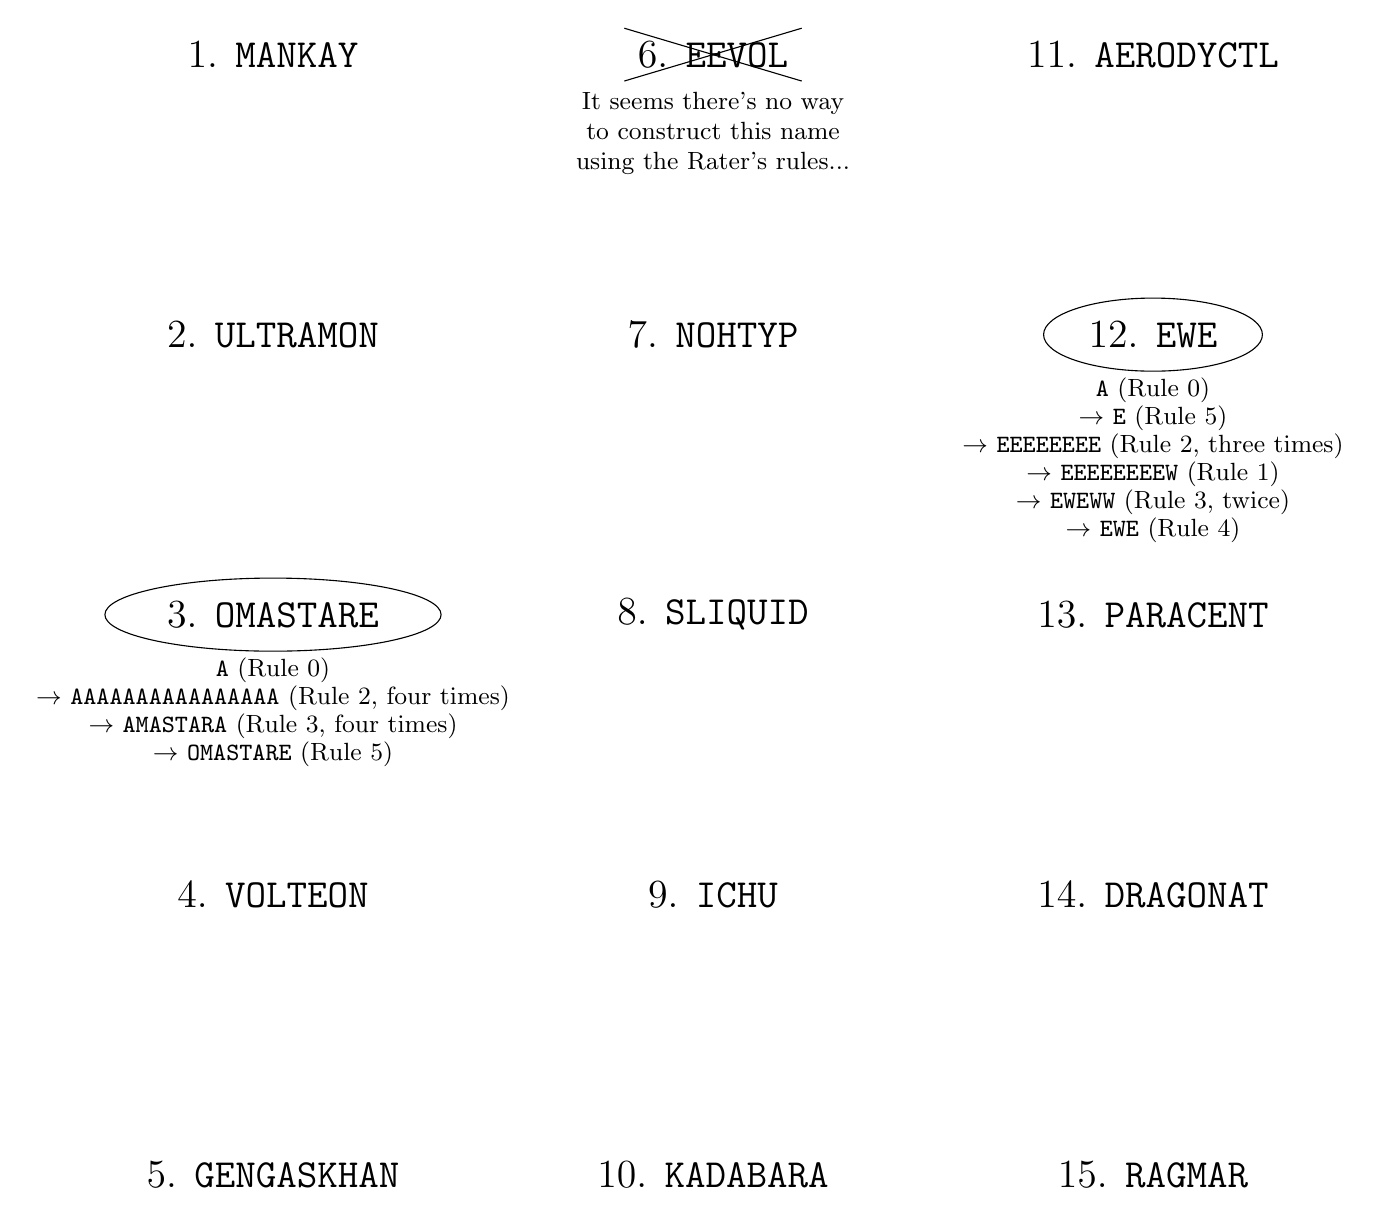
\begin{tikzpicture}[x=2.2in,y=-1.4in]\Large
  \node at (0,0) {1. \texttt{MANKAY}};
  \node at (0,1) {2. \texttt{ULTRAMON}};
  \node[draw,ellipse] at (0,2) {3. \texttt{OMASTARE}};
  \node at (0,3) {4. \texttt{VOLTEON}};
  \node at (0,4) {5. \texttt{GENGASKHAN}};
  
  \node[draw,cross out] at (1,0) {6. \texttt{EEVOL}};
  \node at (1,1) {7. \texttt{NOHTYP}};
  \node at (1,2) {8. \texttt{SLIQUID}};
  \node at (1,3) {9. \texttt{ICHU}};
  \node at (1,4) {10. \texttt{KADABARA}};

  \node at (2,0) {11. \texttt{AERODYCTL}};
  \node[draw,ellipse] at (2,1) {12. \texttt{EWE}};
  \node at (2,2) {13. \texttt{PARACENT}};
  \node at (2,3) {14. \texttt{DRAGONAT}};
  \node at (2,4) {15. \texttt{RAGMAR}};

\small
  \node at (0,2.2) {\texttt{A} (Rule 0)};
  \node at (0,2.3) {\(\rightarrow\) \texttt{AAAAAAAAAAAAAAAA} (Rule 2, four times)};
  \node at (0,2.4) {\(\rightarrow\) \texttt{AMASTARA} (Rule 3, four times)};
  \node at (0,2.5) {\(\rightarrow\) \texttt{OMASTARE} (Rule 5)};

  \node[text width=1.5in,align=center,anchor=north] at (1,0.1) {It seems there's no way to construct this name using the Rater's rules...};

  \node at (2,1.2) {\texttt{A} (Rule 0)};
  \node at (2,1.3) {\(\rightarrow\) \texttt{E} (Rule 5)};
  \node at (2,1.4) {\(\rightarrow\) \texttt{EEEEEEEE} (Rule 2, three times)};
  \node at (2,1.5) {\(\rightarrow\) \texttt{EEEEEEEEW} (Rule 1)};
  \node at (2,1.6) {\(\rightarrow\) \texttt{EWEWW} (Rule 3, twice)};
  \node at (2,1.7) {\(\rightarrow\) \texttt{EWE} (Rule 4)};
\end{tikzpicture}
\end{center}


% Include below for aucTeX integration
%%% Local Variables:
%%% mode: latex
%%% TeX-master: "../mapp-challenge-18-game-book"
%%% End:



%!TEX root =../mapp-challenge-18-game-book.tex
% ^ leave for LaTeXTools build functionality

\phChapterWorksheet{Cross Products}{Cryptic Puzzle 2}

(angry Dojo Master has a mixed up word search like Puzzle A in VBPuzzlehunt)


% Include below for aucTeX integration
%%% Local Variables:
%%% mode: latex
%%% TeX-master: "../mapp-challenge-18-game-book"
%%% End:

%!TEX root =../mapp-challenge-18-game-book.tex
% ^ leave for LaTeXTools build functionality

\phChapterWorksheet{Blind Luck}{Strange Tilework}

\begin{center}
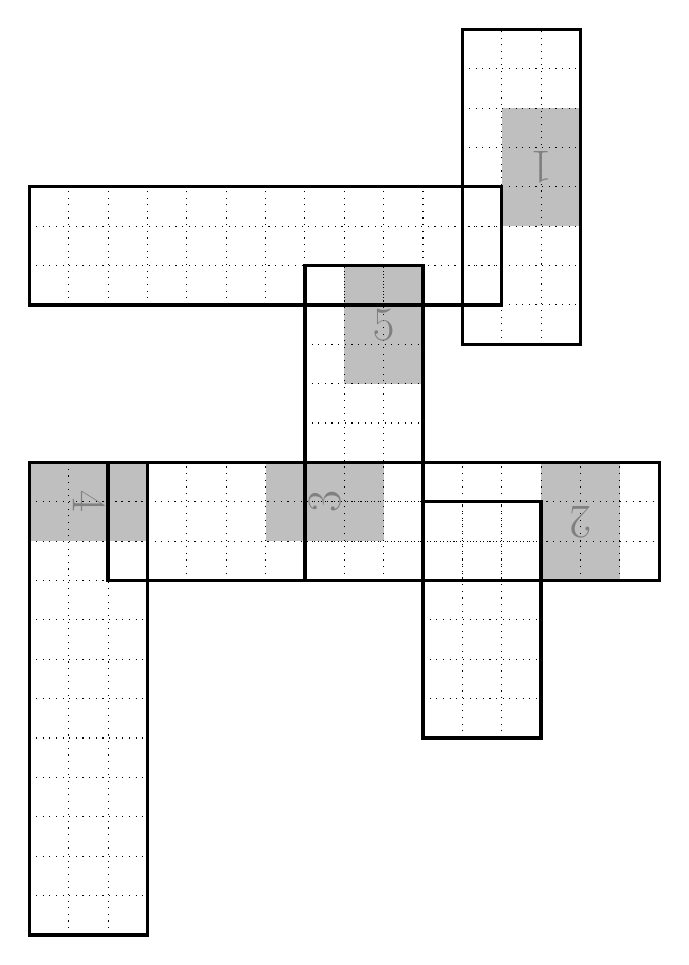
\begin{tikzpicture}[x=0.5cm,y=0.5cm]
  \fill[color=lightgray] (8,14) rectangle (10,17);
  \fill[color=lightgray] (0,10) rectangle (3,12);
  \fill[color=lightgray] (6,10) rectangle (9,12);
  \fill[color=lightgray] (13,9) rectangle (15,12);
  \fill[color=lightgray] (12,18) rectangle (14,21);

  \blindCrissCrossEntry{(0,0)}{(3,12)};
  \blindCrissCrossEntry{(2,9)}{(16,12)};
  \blindCrissCrossEntry{(10,5)}{(13,11)};
  \blindCrissCrossEntry{(7,9)}{(10,17)};
  \blindCrissCrossEntry{(0,16)}{(12,19)};
  \blindCrissCrossEntry{(11,15)}{(14,23)};

  \node at (9,15.5) {\LARGE\rotatebox{0}{\textcolor{gray}{5}}};
  \node at (1.5,11) {\LARGE\rotatebox{-90}{\textcolor{gray}{4}}};
  \node at (7.5,11) {\LARGE\rotatebox{90}{\textcolor{gray}{3}}};
  \node at (14,10.5) {\LARGE\rotatebox{180}{\textcolor{gray}{2}}};
  \node at (13,19.5) {\LARGE\rotatebox{180}{\textcolor{gray}{1}}};
\end{tikzpicture}
\end{center}


% Include below for aucTeX integration
%%% Local Variables:
%%% mode: latex
%%% TeX-master: "../mapp-challenge-18-game-book"
%%% End:


\phPart{Game Control Documents}

\phChapter{Printing instructions}
\begin{itemize}
\item A copy of the \textbf{Player Handout} section of this PDF should
be printed and stapled for each participant, using the PDF title page
as the cover.

\item The six \textbf{Knot True Badges} should be printed and laminated
for display during the Opening Puzzle.
Extras should also be available as backups (lamination optional).

\item Several \textbf{ClueKeeper Reference} packets should be printed
and compiled for use by Game Control, and to hand out in case
players cannot install ClueKeeper for the demo.
\end{itemize}


\phChapterWorksheet{Knot True}{Ash's Trainer Badge}

  \begin{center}
    \includegraphics[width=4in]{assets/unknot1.pdf}

    \Huge Trainer ID: 365867

%    Ash and Flannery did not place 6th.
  \end{center}

\phWorksheet{Brock's Trainer Badge}
  \begin{center}

    \includegraphics[width=4in]{assets/knot1.pdf}

    \Huge Trainer ID: 198815
%
%    Neither Brock nor Drayden placed 4th.
%
%
  \end{center}

\phWorksheet{Cynthia's Trainer Badge}
  \begin{center}
    \includegraphics[width=4in]{assets/unknot2.pdf}

    \Huge Trainer ID: 255123 
%
%    Erika placed exactly one rank higher than Ash.
%
  \end{center}

\phWorksheet{Drayden's Trainer Badge}
  \begin{center}
%
    \includegraphics[width=4in]{assets/knot2.pdf}

    \Huge Trainer ID: 443881 
%
%    Drayden placed in the top three.
%
%
  \end{center}

\phWorksheet{Erika's Trainer Badge}
  \begin{center}
    \includegraphics[width=4in]{assets/knot3.pdf}

    \Huge Trainer ID: 310235 
%
%    Brock placed lower than Flannery.
%
%
  \end{center}

\phWorksheet{Flannery's Trainer Badge}
  \begin{center}
    \includegraphics[width=4in]{assets/unknot3.pdf}

    \Huge Trainer ID: 663968
%
%    Either Cynthia or Drayden placed 3rd.
  \end{center}


\phChapter{Cluekeeper Reference}

\phSection{Knot True -- Introduction}

In a recent Mob\'imon tournament, six Mob\'imon trainers were ranked from 1st to 6th:

\begin{multicols}{3}
\begin{itemize}
\item Ash
\item Brock
\item Cynthia
\item Drayden
\item Erika
\item Flannery
\end{itemize}
\end{multicols}

To prove to your mentor, Professor Sassafras, that you are ready to embark on your Mob\'imon adventure, she has tasked you with finding these six trainers and ask them what they remember about the tournament results.

To obtain their six clues, look for six \textbf{Trainer Badges} found on posters located nearby, and enter the \textbf{Trainer ID} shown for each into ClueKeeper.

\vfill

\phSection{Knot True -- Clues unlocked by each badge}

\begin{multicols}{3}\footnotesize
  \begin{center}
    \includegraphics[width=1.2in]{assets/unknot1.pdf}

    Ash and Flannery did not place 6th.


    \includegraphics[width=1.2in]{assets/knot1.pdf}

    Neither Brock nor Drayden placed 4th.


    \includegraphics[width=1.2in]{assets/unknot2.pdf}

    Erika placed exactly one rank higher than Ash.


    \includegraphics[width=1.2in]{assets/knot2.pdf}

    Drayden placed in the top three.


    \includegraphics[width=1.2in]{assets/knot3.pdf}

    Brock placed lower than Flannery.


    \includegraphics[width=1.2in]{assets/unknot3.pdf}

    Either Cynthia or Drayden placed 3rd.
  \end{center}
\end{multicols}

\newpage

\phSection{Knot True -- Final clue unlocked by collecting badges}

Wait a second... it seems that not all of the six trainers are telling the truth! You'll need to determine which of the trainers are lying by inspecting their trainer badges. If the cord shown in a badge can be tightened into a knot, then that trainer is lying; if not, they are telling the truth!

Use the clues associated with each Trainer Badge and the provided \textbf{Tournament Results} 
page to mark how each trainer placed in the tournament. Doing so correctly will reveal a word. 
Enter this word into ClueKeeper to prove to Professor Sassafras that you're ready to begin your 
Mob\'imon adventure!

\vfill

\phSection{When Push Comes to Shove -- Main Puzzle 1}

While training your Mob\'imon near the wharf, you lock eyes with Dockworker Dave. As everyone knows, when two trainers' eyes meet, it's time for a Mob\'imon battle!

You're still a beginner though, so you manage to talk him down to a puzzle. Dave agrees, and shows you the image shown below. He explains that this illustration demonstrates the seven different ways that five boxes can be stacked flush against the wall of his warehouse.

It seems that some rat Mob\'imon have thrown the warehouse into disarray, so you'll need to help Dave calculate how many different ways his boxes can be rearranged according to the criteria shown on the provided 
\textbf{Warehouse Specifications} sheet. Calculating these possibilities and using the encoding A=1, B=2, etc. will reveal the solution to this puzzle!

\newcommand{\mappBoxRow}[2]{
  \fill[color=lightgray] #1 rectangle #2;
  \draw[step=1]          #1 grid #2;
}
\begin{center}
  \begin{tikzpicture}[x=0.15in,y=0.15in]
    \mappBoxRow{(0,0)}{(5,1)}

    \draw[thick] (0,0) -- (0, 5);
    \draw[thick] (0,0) -- (5, 0);
  \end{tikzpicture}
  \begin{tikzpicture}[x=0.15in,y=0.15in]
    \mappBoxRow{(0,0)}{(4,1)}
    \mappBoxRow{(0,1)}{(1,2)}

    \draw[thick] (0,0) -- (0, 5);
    \draw[thick] (0,0) -- (5, 0);
  \end{tikzpicture}
  \begin{tikzpicture}[x=0.15in,y=0.15in]
    \mappBoxRow{(0,0)}{(3,1)}
    \mappBoxRow{(0,1)}{(2,2)}

    \draw[thick] (0,0) -- (0, 5);
    \draw[thick] (0,0) -- (5, 0);
  \end{tikzpicture}
  \begin{tikzpicture}[x=0.15in,y=0.15in]
    \mappBoxRow{(0,0)}{(3,1)}
    \mappBoxRow{(0,1)}{(1,2)}
    \mappBoxRow{(0,2)}{(1,3)}

    \draw[thick] (0,0) -- (0, 5);
    \draw[thick] (0,0) -- (5, 0);
  \end{tikzpicture}
  \begin{tikzpicture}[x=0.15in,y=0.15in]
    \mappBoxRow{(0,0)}{(2,1)}
    \mappBoxRow{(0,1)}{(2,2)}
    \mappBoxRow{(0,2)}{(1,3)}

    \draw[thick] (0,0) -- (0, 5);
    \draw[thick] (0,0) -- (5, 0);
  \end{tikzpicture}
  \begin{tikzpicture}[x=0.15in,y=0.15in]
    \mappBoxRow{(0,0)}{(2,1)}
    \mappBoxRow{(0,1)}{(1,2)}
    \mappBoxRow{(0,2)}{(1,3)}
    \mappBoxRow{(0,3)}{(1,4)}

    \draw[thick] (0,0) -- (0, 5);
    \draw[thick] (0,0) -- (5, 0);
  \end{tikzpicture}
  \begin{tikzpicture}[x=0.15in,y=0.15in]
    \mappBoxRow{(0,0)}{(1,1)}
    \mappBoxRow{(0,1)}{(1,2)}
    \mappBoxRow{(0,2)}{(1,3)}
    \mappBoxRow{(0,3)}{(1,4)}
    \mappBoxRow{(0,4)}{(1,5)}

    \draw[thick] (0,0) -- (0, 5);
    \draw[thick] (0,0) -- (5, 0);
  \end{tikzpicture}
\end{center}

\vfill

\newpage

\phSection{The Nickname Rater -- Main Puzzle 2}

As your adventure continues, you find yourself in
Achromatopsia City,
home of the famous \mappMobimon{} Nickname Rater.
She explains that while Trainers often like to give their
\mappMobimon{} cute nicknames, she's very particular about the rules
for an ``excellent'' \mappMobimon{} nickname.

\begin{multicols}{2}
\begin{itemize}
  \item \textbf{Rule 0:}
        \texttt{A} is an excellent nickname.
  \item \textbf{Rule 1:}
        Adding a consonant to the end of an excellent nickname ending with
        a vowel creates a new excellent nickname.
  \item \textbf{Rule 2:}
        Doubling an excellent nickname creates a new excellent nickname.
  \item \textbf{Rule 3:}
        Replacing three consecutive vowels in an excellent nickname with
        a consonant creates a new excellent nickname.
  \item \textbf{Rule 4:}
        Removing two consecutive consonants from an excellent nickname
        creates a new excellent nickname.
  \item \textbf{Rule 5:}
        Exchanging the consonants in an excellent nickname with other
        consonants creates a new excellent nickname. Similarly,
        exchanging the vowels in an excellent nickname with other vowels
        creates a new excellent nickname.
  \item Nicknames that cannot be created using these rules are not
        excellent.
\end{itemize}
\end{multicols}

The Nickname Rater suggests you try rating the nicknames shown on the provided 
\textbf{Popular Nicknames} sheet. Apparently if you take the first letters of the excellent nicknames in order, you can spell a great (but not excellent) seven-letter word for a nickname.

\vfill

\phSection{Cross Product -- Cryptic Puzzle 1}

Impressed with your problem-solving ability, the dockworker suggests you head to the \mappMobimon{} Dojo. There, the Dojo Master agrees to battle you, but only if you can solve his puzzle. He presents you a copy of an 
\textbf{Odd Scroll} and the following clues:

\begin{itemize}
\item \textit{Only a trainer that has one of these can possibly become HIPCONAM.}
\begin{itemize}
\item Lightning \(\times\) Plant
\item Undead \(\times\) Flame 
\item Aqua \(\times\) Ordinary
\item Flame \(\times\) Magic
\end{itemize}
\end{itemize}

Can you \textit{unscramble} the meaning of the Dojo Master's scroll, putting you one step closer to becoming a \mappMobimon{} Champion?

\vfill

\newpage

\phSection{Blind Luck -- Cryptic Puzzle 2}

The Nickname Rater suggests you continue your journey just down the road, where the sightless Dojo Master is known to battle up-and-coming Mob\'imon trainers.

You arrive at the dojo, but it seems that a secret
password is required to enter, and your only clue is the \textbf{Strange Tilework} leading to the dojo's door.

After scratching your head for a bit, you lean against the door. You hear a low whisper carry the following words into your ear:

\begin{itemize}
\item RED
\item BLUE
\item YELLOW
\item GOLD
\item SILVER
\item CRYSTAL
\end{itemize}


Are these the clues you need to figure out the secret password?

\end{document}

%%% Local Variables:
%%% mode: latex
%%% TeX-master: t
%%% End:
